% !TeX root = ../tesis.tex



%
\begin{figure}[h!]
\def\svgwidth{\textwidth} \small
\hspace*{.75em}
\begin{subfigure}{.1\textwidth}\caption{ }\label{sfig:red:1}\end{subfigure}
\vspace*{12.5em} % Crece la distancia entre as etiquetas
\\
\vspace*{-16.5em} % Crece la distancia entre las etiquetas y el pie de figura
\hspace*{0.5em}%
\begin{subfigure}{.1\textwidth}\caption{ }\label{sfig:red:2}\end{subfigure}\\
\includeinkscape{1-Theory-Figs/0-NoConv/0-NoConv}
\vspace*{-2em} %Crece la ditancia entre la imagen y el pie de figura
\caption[Spectral redshift of the scattering and extinciton of a spherical AuNP as function of its size and the embedding media]{Resonance wavlength ($\lambda_\text{res}$) of the scattering (orange) and extinction (black) cross sections as functions of the NPs radii when embedded  \ref{sfig:red:1} into air and \ref{sfig:red:2} into water, and as function of the refractive index of the matrix for NP of radius set to  \ref{sfig:red:3} 12.5 nm and \ref{sfig:red:4} 50 nm.}
\end{figure}


%
\begin{figure}[h!]\centering
	\def\svgwidth{.8\textwidth} \small
\includeinkscape{1-Theory-Figs/1-RadiusConv/1-RadiusConv}
\vspace*{-1em}
\caption[Spectral redshift of the scattering and extinciton of a spherical AuNP as function of its size and the embedding media]{Resonance wavlength ($\lambda_\text{res}$) of the scattering (orange) and extinction (black) cross sections as functions of the NPs radii when embedded  \ref{sfig:red:1} into air and \ref{sfig:red:2} into water, and as function of the refractive index of the matrix for NP of radius set to  \ref{sfig:red:3} 12.5 nm and \ref{sfig:red:4} 50 nm.}
\end{figure}

%
\begin{figure}[h!]\centering
	\def\svgwidth{.8\textwidth} \small
\includeinkscape{1-Theory-Figs/2-MatrixConv/2-MatrixConv}
\vspace*{-1em}
\caption[Spectral redshift of the scattering and extinciton of a spherical AuNP as function of its size and the embedding media]{Resonance wavlength ($\lambda_\text{res}$) of the scattering (orange) and extinction (black) cross sections as functions of the NPs radii when embedded  \ref{sfig:red:1} into air and \ref{sfig:red:2} into water, and as function of the refractive index of the matrix for NP of radius set to  \ref{sfig:red:3} 12.5 nm and \ref{sfig:red:4} 50 nm.}
\end{figure}

















%
\begin{figure}\centering
%\def\svgwidth{\textwidth} \small
%\includeinkscape{2-Results-Figs/redshift/redshift}%
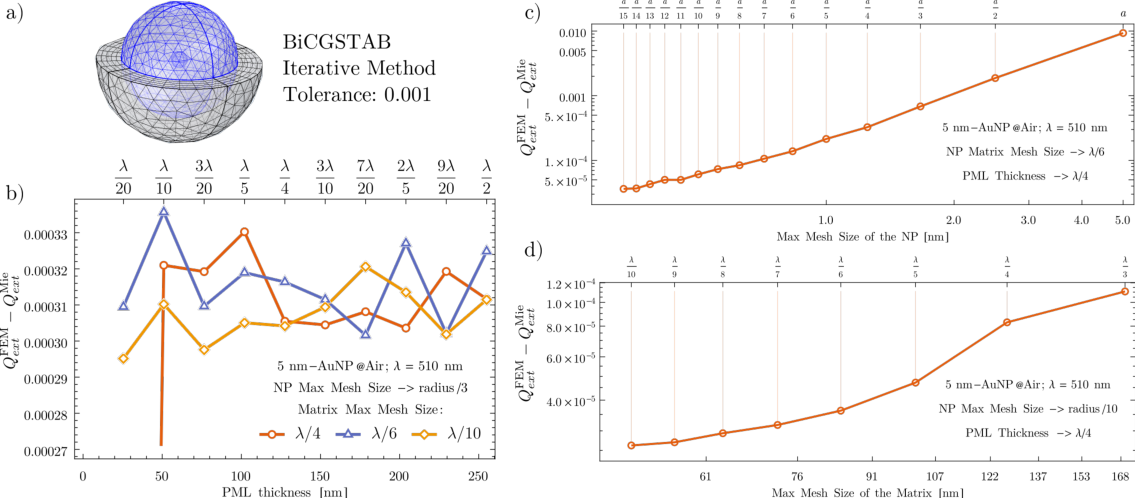
\includegraphics[scale = .8 ]{1-Theory-Figs/drawingCOMSOL.pdf}
\caption[Convergence tests: The Meshing]{Resonance wavlength ($\lambda_\text{res}$) of the scattering (orange) and extinction (black) cross sections as functions of the NPs radii when embedded  \ref{sfig:red:1} into air and \ref{sfig:red:2} into water, and as function of the refractive index of the matrix for NP of radius set to  \ref{sfig:red:3} 12.5 nm and \ref{sfig:red:4} 50 nm.}
\end{figure}

\clearpage

\begin{figure}\centering
%\def\svgwidth{\textwidth} \small
%\includeinkscape{2-Results-Figs/redshift/redshift}%
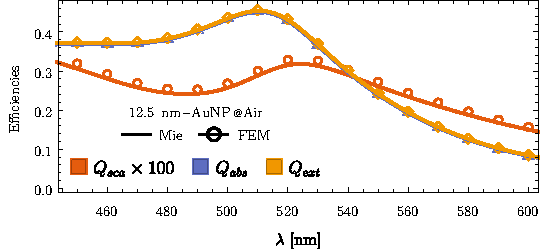
\includegraphics[width = .8\textwidth ]{1-Theory-Figs/Mie-FEM_Air.pdf}\\
\includegraphics[width = .4\textwidth ]{1-Theory-Figs/Isolated-COMSOL.pdf}%
\includegraphics[width = .4\textwidth ]{1-Theory-Figs/Isolated-COMSOL.pdf}%
\caption[Convergence tests: The Meshing]{Resonance wavlength ($\lambda_\text{res}$) of the scattering (orange) and extinction (black) cross sections as functions of the NPs radii when embedded  \ref{sfig:red:1} into air and \ref{sfig:red:2} into water, and as function of the refractive index of the matrix for NP of radius set to  \ref{sfig:red:3} 12.5 nm and \ref{sfig:red:4} 50 nm.}
\end{figure}
